\section{Frozen Interim Depth Models: Actual Coded Rate}
\label{sec:interimdepth}

The four-crop health monitor cannot establish a rate--distortion frontier.
We therefore freeze the D2, D4 and D6 checkpoints after exactly 20 of the
105 scheduled epochs and evaluate all 100 DIV2K validation images as
$512\times512$ centre crops. The released D12 checkpoint is a practical
anchor with different training provenance, not the control that isolates
the effect of depth. All four models are evaluated at QPs 0, 16, 32, 48
and 63: 2,000 encode/decode cases. No checkpoint is selected using these
results. The study is an interim diagnostic, not the final depth ablation.
We repeat the complete protocol at the fixed epoch-30 milestone below;
the plotted geometry and allocation controls retain their epoch-20 weights.

\paragraph{A causal CPU reference.}
Each stream contains actual rANS payload. An encoder-independent process
reconstructs the image using the stream and resident model, with source
analysis disabled. It first decodes the hyperlatent and then the four
causal main-latent stages; entropy indexes come from the decoder's recovered
context, rather than being supplied by the encoder. Every case has exact
reconstruction, latent and symbol/index-trace checks. The decoder process
is reused within a model, so independence does not imply a newly launched
process for every image. The reference uses CPU FP32 and a versioned
research format, not the released CUDA FP16 format or a latency benchmark.

We distinguish entropy estimates, rANS payload and container bytes.
The research header is 88 bytes per crop, including 64 bytes of identity
and integrity hashes: 0.002686\,bpp on a $512^2$ crop. This is not a
minimal production header or the cost of a routing map. Reconstructions
are explicitly converted from clipped YCbCr to clipped RGB before quality
measurement. These RGB results are separate from the legacy shared-exit
archive's equal-channel YCbCr-MSE metric.

\paragraph{Compare rate, not quality index.}
For each image, we interpolate PSNR linearly in log payload rate and retain
only the common support of all four codecs. No quality is extrapolated.
The supported cohorts contain 95, 99 and 89 images at 0.1, 0.2 and
0.4\,bpp respectively. At 0.2\,bpp, D4 and D6 improve over D2 by
0.1207\,dB [0.1018, 0.1420] and 0.1834\,dB [0.1572, 0.2115]; the released
D12 gap is 0.6986\,dB [0.5989, 0.8112]. Intervals use 5,000 paired-image
bootstrap draws, conditional on the fixed checkpoints and included images.
They do not measure training-seed variation. PCHIP interpolation gives
0.1209, 0.1839 and 0.6880\,dB on the same 99-image support.
\Cref{fig:interimdepth} separates native-QP population means from these
paired, equal-rate comparisons.

\begin{figure*}[t]
\centering
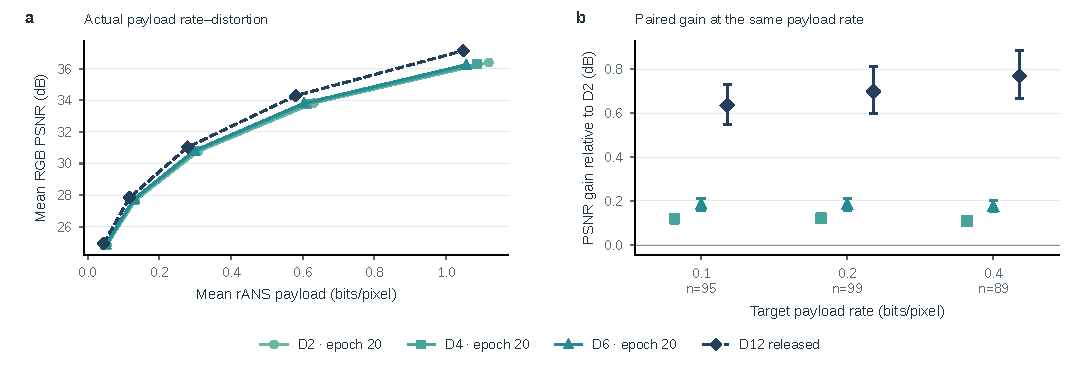
\includegraphics[width=\textwidth]{figs/research20260927/div2k100_epoch020/fig_reference_rd.pdf}
\caption{\textbf{Shallow models are close, but not identical, at equal coded rate.}
\textbf{a}, Mean RGB PSNR and actual payload over all 100 crops at five QPs;
joining lines are visual guides. \textbf{b}, Per-image interpolation and
paired differences on four-model common support, with 95\% image-bootstrap
intervals. D2/D4/D6 are frozen epoch-20 models; released D12 is not matched
in training history. These measured streams establish an interim CPU
rate--distortion comparison, not final quality or native runtime.}
\label{fig:interimdepth}
\end{figure*}

\paragraph{Why the small monitor was insufficient.}
The original four crops and the additional 96 are reported separately on
the same supported cohort (\cref{fig:interimcoverage}). The four-crop
subset overstates the mean depth advantage at 0.2\,bpp; it is useful for
training health, not a substitute for the validation distribution.
D6 nevertheless retains an approximately 0.18\,dB mean advantage over
D2 across the larger cohort. Its modest magnitude is therefore not solely
an artefact of monitoring four images. The remaining released-model gap
cannot be attributed to depth until an official-recipe D12 control has
been trained for the same schedule.

\begin{figure*}[t]
\centering
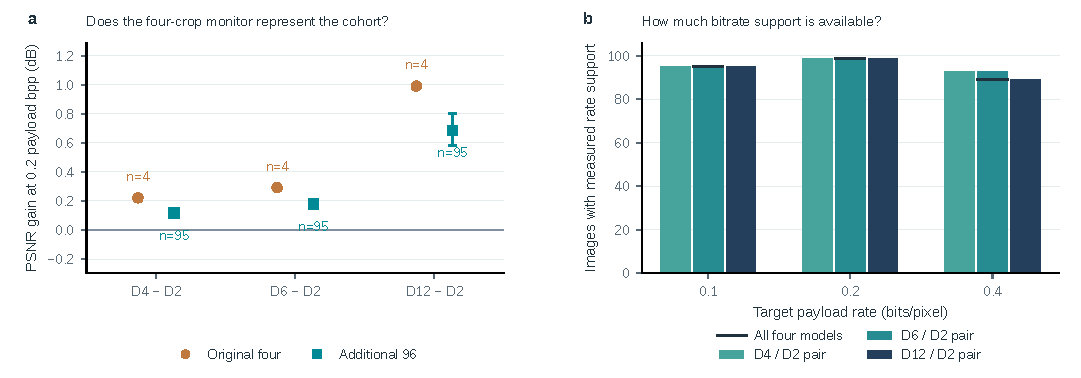
\includegraphics[width=\textwidth]{figs/research20260927/div2k100_epoch020/fig_reference_coverage.pdf}
\caption{\textbf{Coverage is part of the result.}
\textbf{a}, Original monitor crops and additional images at 0.2 payload bpp,
restricted to four-model common support. We do not estimate uncertainty
from the four-crop subset. \textbf{b}, Pairwise and four-model supported
counts at each target rate. A changing cohort is made explicit rather than
filled by extrapolation.}
\label{fig:interimcoverage}
\end{figure*}

BD-rate is computed per image using PCHIP interpolation of log rate as a
function of PSNR, over the intersection of all four models' PSNR ranges.
All 100 images have a valid interval. Relative to released D12, mean payload
BD-rate is +21.56\% for D2, +17.84\% for D4 and +15.69\% for D6
(\cref{fig:interimbytes}). This compares unfinished shallow models with a
released checkpoint; it is not the bitrate penalty caused by truncation
at matched convergence. Averaging per-image BD-rate and comparing
population-mean RD curves are different estimands.

\begin{figure*}[t]
\centering
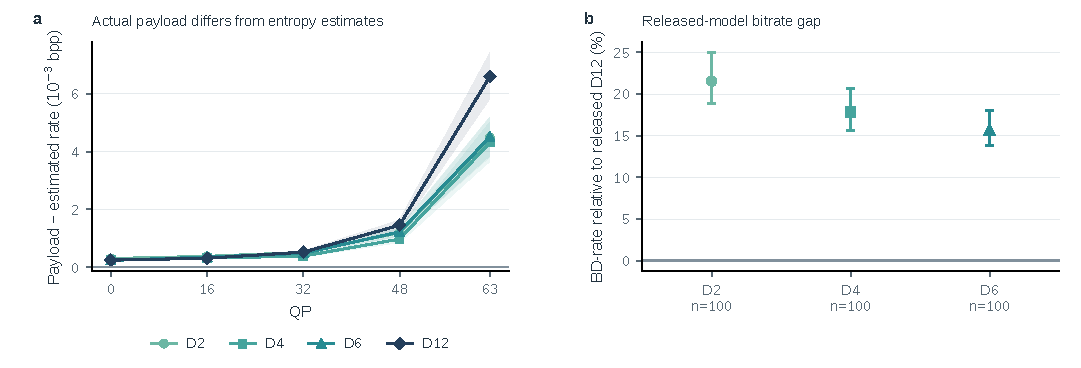
\includegraphics[width=\textwidth]{figs/research20260927/div2k100_epoch020/fig_reference_rate_accounting.pdf}
\caption{\textbf{Estimated entropy and emitted bytes are separate quantities.}
\textbf{a}, Actual rANS payload minus entropy estimate, excluding the research
header. \textbf{b}, Mean per-image BD-rate against the released anchor on
each image's four-model common PSNR interval. Intervals resample images;
no uncertainty from independent training seeds is represented.}
\label{fig:interimbytes}
\end{figure*}

\paragraph{Milestone sensitivity.}
The next fixed checkpoint at epoch 30 repeats all 2,000 encode/decode
cases. The crop manifest, CPU backend and research format are unchanged;
all 500 released-D12 measurements reproduce exactly. To compare depth
ordering, \cref{fig:milestones} retains the same 99 images on common
0.2-payload-bpp support across both milestones and all four models.
D6's mean advantage over D4 changes from 0.0627\,dB to
$-0.0045$\,dB, whose interval includes zero. Relative to their own
epoch-20 curves, D2 and D4 gain 0.0259 and 0.0168\,dB while D6 loses
0.0504\,dB on this support. These are descriptive checkpoint differences,
not evidence that training a deeper model is intrinsically harmful.
Both milestones are retained without quality-based checkpoint selection;
neither establishes the final ordering after 105 epochs.

\begin{figure}[t]
\centering
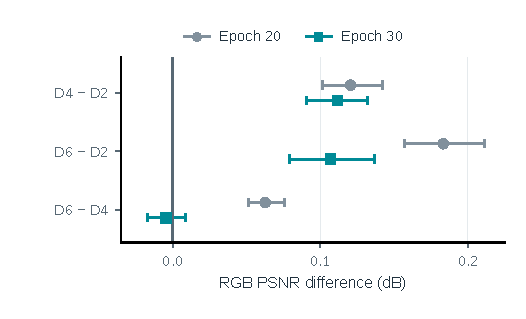
\includegraphics[width=\columnwidth]{figs/editorial20260928/fig_depth_milestones.pdf}
\caption{\textbf{Intermediate depth ordering changes during training.} Paired RGB PSNR differences at 0.2 actual payload bpp on the same 99 images. Epochs 20 and 30 are retained without quality-based selection. Intervals are 95\% image-bootstrap intervals at fixed weights, excluding training-seed uncertainty. No rate extrapolation.}
\label{fig:milestones}
\end{figure}

\section{Does an Additional Expert Add an Additional Choice?}

A bank with more models has greater capacity, but the value of its middle
experts depends on the attainable allocation frontier. We perform a
conditional leave-D4-out analysis on the measured epoch-20 D2/D4/D6 curves.
The decision unit is a whole $512^2$ crop, not a patch within an image.
All three choices are compared at the same interpolated payload rate for
each image. Dynamic programming minimises summed RGB MSE under an aggregate
neural-decoder Conv2d MAC budget, permitting unused budget. The objective is
reported as PSNR of pooled MSE, not mean per-image PSNR.

\Cref{fig:interimallocation} separates two questions. Removing D4 measures
its incremental option value relative to the best D2/D6 assignment.
Permuting the labels of the best source-calibrated blind histogram measures
the value of knowing where to place depth. The blind comparator minimises
expected MSE on this same cohort; it is deliberately optimistic and is not
a deployable validation-fitted policy. At a budget equal to uniform D4,
adding D4 is worth 0.0132, 0.0086 and 0.0061\,dB at 0.1, 0.2 and
0.4\,bpp. Source-informed placement over the blind expectation is worth
0.0239, 0.0303 and 0.0299\,dB. These are deterministic, conditional bounds
at one interim checkpoint. They motivate expert-removal controls, rather
than establishing that a six-expert spatial bank is necessary.

\begin{figure*}[t]
\centering
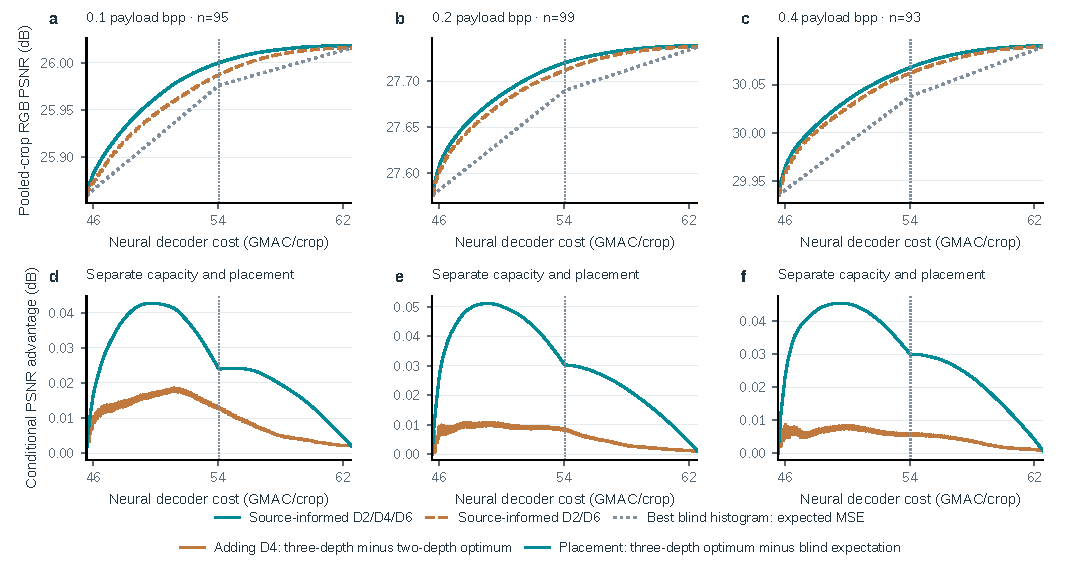
\includegraphics[width=\textwidth]{figs/research20260927/depth_allocation/fig_depth_allocation.pdf}
\caption{\textbf{Separate the value of capacity choices from their assignment.}
Top: exact whole-crop allocation under a shared neural-decoder MAC budget.
Bottom: incremental D4 option value and assignment premium over the best
source-calibrated blind histogram's expected MSE. Vertical guides mark the
uniform-D4 budget. The curves use interpolated equal-rate quality and
contain neither patch entropy resets nor a trained MLP. They are not
within-image routing results or runtime frontiers.}
\label{fig:interimallocation}
\end{figure*}

\paragraph{Complexity is not the training target.}
We also report every combination of three cheap source statistics, two
depth comparisons and three rates: RGB standard deviation, gradient energy
and Laplacian energy versus D4--D2 or D6--D2 benefit
(\cref{fig:interimfeatures}). At 0.2\,bpp, gradient energy has Spearman
correlation 0.270 with D4--D2 but only 0.111 with D6--D2; Laplacian energy
has correlation 0.011 with D6--D2. This does not rule out a learned cheap
representation. It does caution against treating visible texture as a
sufficient label for incremental reconstruction benefit. The statistics
are descriptive associations on development-used data, without significance
selection or held-out prediction claims. A later selector must be trained
and assessed on separate images using rate, distortion and measured cost.

\begin{figure*}[t]
\centering
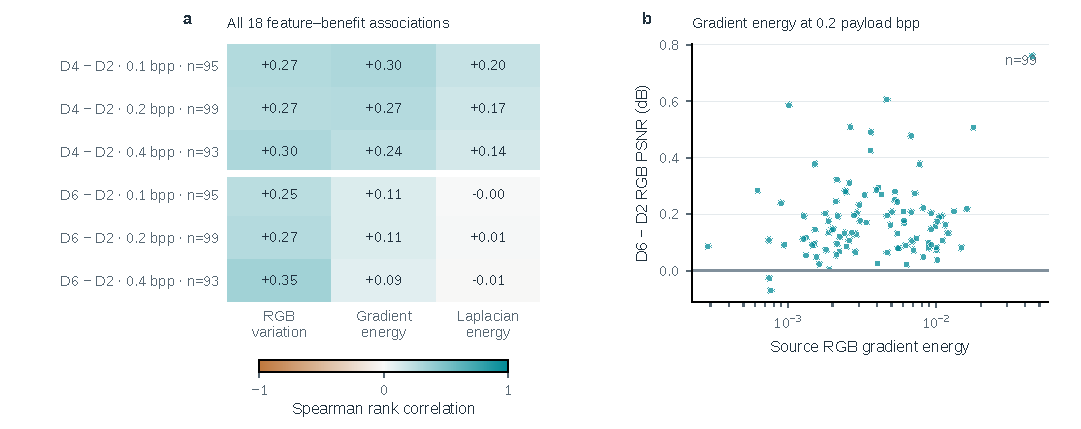
\includegraphics[width=\textwidth]{figs/research20260927/source_features/fig_source_depth_association.pdf}
\caption{\textbf{Cheap complexity measures do not directly identify the useful expert.}
All 18 specified feature/depth/rate combinations are shown, with supported
image counts. The scatter panel was fixed to gradient energy versus D6--D2
at 0.2\,bpp before inspecting the associations. These are correlations with
interim equal-rate benefits, not router accuracy or causal feature effects.}
\label{fig:interimfeatures}
\end{figure*}
